\documentclass[a4paper,twocolumn,10pt]{ltjsarticle}
\usepackage[margin=25mm,left=20mm,right=20mm]{geometry}
\usepackage{graphicx}
\usepackage{booktabs}
\pagestyle{empty}
\setlength{\columnsep}{10mm}
\title{\textbf{カテゴリ別プロファイル切り替え機構を備えたPatchCore-lite異常検知システムのFPGA実装に向けた検討}}
\author{山田 峻也・高木 一義\\ 三重大学大学院 工学研究科 情報工学専攻 コンピュータアーキテクチャ研究室\\ （E-mail: shunya@arch.info.mie-u.ac.jp）}
\date{}
\begin{document}
\maketitle
\begin{abstract}
PatchCoreは，正常画像から得た特徴量をメモリバンクとして保持し，推論時に入力特徴量と正常特徴量の距離を近傍探索で求める異常検知手法である。高い検知性能を持つ一方で，複数カテゴリを一つの装置で扱う場合，共通設定では現在検査しているカテゴリに不要な特徴量やメモリバンクまで探索し，FPGA実装時のメモリアクセスと探索回数が大きくなる。本稿では，共通CNNを維持しつつ，検査カテゴリごとに特徴層，グリッド，top-k，しきい値，メモリバンク参照範囲を切り替えるPatchCore-lite異常検知システムを検討する。MVTec ADを用いた予備実験では，欠陥誤通過率を一定以下に制約した条件で，良品通過率を保ちながら近傍探索量を削減できることを確認した。
\end{abstract}
\noindent\textbf{キーワード:} 産業用異常検知，PatchCore，FPGA，近傍探索，プロファイル切り替え
\section*{1. はじめに}
工業検品では，欠陥品を良品として通してしまう誤通過を抑えつつ，良品をできるだけ多く通過させることが求められる。PatchCore[1]は正常例のみから学習でき，MVTec AD[2]などで高い異常検知性能が報告されているため，検品システムの土台として有力である。一方で，PatchCoreの推論ではCNNによる特徴抽出に加えて，正常特徴量を保存したメモリバンクとのk近傍探索（KNN探索）が必要になる。

複数カテゴリを一つのFPGAで扱う場合，全カテゴリ共通の設定と共通メモリバンクを用いる構成が考えられる。しかしこの構成では，現在検査しているカテゴリに不要な正常特徴まで探索する。また，カテゴリごとに有効な特徴層やグリッド密度が異なる場合でも，同じ設定を用いる必要がある。本研究では，カテゴリ情報が検査前に分かっている状況を利用し，FPGA内部の動作モードをカテゴリごとに切り替える構成を検討する。

\section*{2. PatchCore}
PatchCore[1]は，正常画像の特徴量を記憶しておき，入力画像がその正常特徴からどれだけ離れているかで異常を検知する手法であり，その処理流れを図1に示す。まず，入力画像からバックボーンCNNによって中間特徴マップを抽出する。次に，その特徴マップをパッチ単位の特徴ベクトルへ変換する。学習時には正常画像から得られた特徴ベクトルだけをメモリバンクに保存し，推論時には入力特徴とメモリバンクの距離を近傍探索で計算する。入力特徴が正常特徴から大きく離れていれば異常と判定する。

PatchCoreで主に設定できる要素は，バックボーンCNN，profile，メモリバンクである。バックボーンCNNはWideResNet50-2などの特徴抽出器であり，画像から特徴マップを取り出す。profileは，CNN後段で用いる軽量な設定群を指す。layer2/layer3は利用するCNN中間特徴層，grid 14は特徴マップを14 x 14個のパッチ位置として扱う設定，Dは各パッチ特徴ベクトルの次元数，top-kは画像全体の異常スコアを作る際に上位何割のパッチ異常スコアを使うかを表す。

メモリバンクは，正常画像から得た代表的なパッチ特徴を保存する領域である。バンクを大きくすると正常分布を広く覆えるが，推論時のメモリ読み出し量とKNN探索回数が増える。そこでPatchCoreでは，正常特徴を代表する点だけを残すk-center coresetが広く使われる[1][3]。本評価では，カテゴリ別profile切り替えの効果を分離するため，全ての比較構成で同じcoreset条件とbank数を用いる。

\begin{figure}[h]
\centering
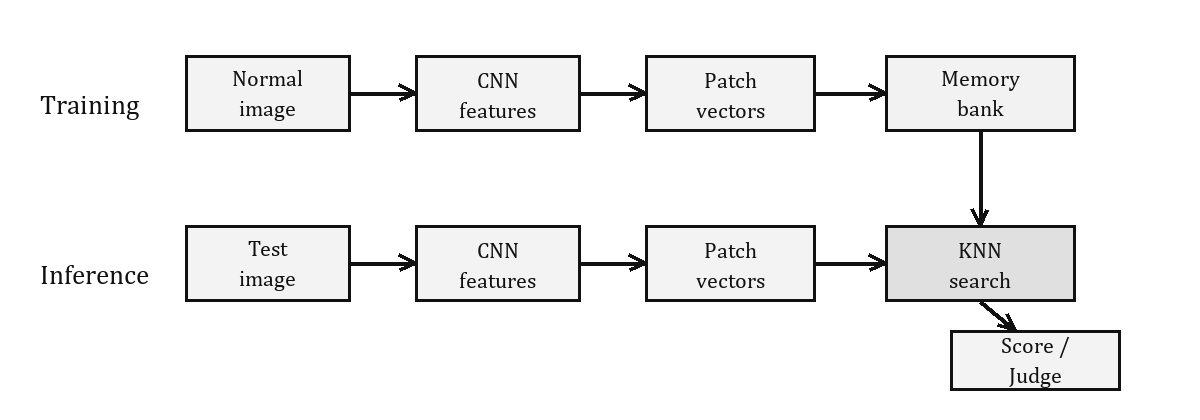
\includegraphics[width=\columnwidth]{figures/patchcore_process.png}
\caption{PatchCoreの学習時・推論時の処理流れ}
\end{figure}
\section*{3. 提案手法}
提案手法は，複数カテゴリを一つのFPGAで検査する状況を対象とし，構成を図2に示す。CNNの主要なデータパスは一つだけ用意し，検査カテゴリに応じてprofileレジスタとメモリバンク参照範囲を切り替える。切り替える値は，特徴層，グリッドサイズ，特徴次元，top-k集約，異常判定しきい値，カテゴリ別bankの開始アドレスと探索長である。これは画像ごとに別の推論モデルを動かす構成ではなく，検査対象が切り替わる直前に動作モードを更新する構成である。

提案手法の特徴は，既存のメモリバンク削減に加えて，カテゴリごとに実行時のprofileを切り替える点にある。既存のPatchCore高速化では，k-center coresetにより保存する正常特徴量を削減する[1][3]。本研究ではさらに，検査ラインで事前に得られるカテゴリ情報を用いて，現在のカテゴリに対応した特徴層，集約方法，bank参照範囲を選択する。これにより，全カテゴリ共通PatchCoreより探索活動量を減らしつつ，カテゴリごとに完全に別のPatchCore回路を用意する場合より主要回路を共有できる。

\begin{figure}[h]
\centering
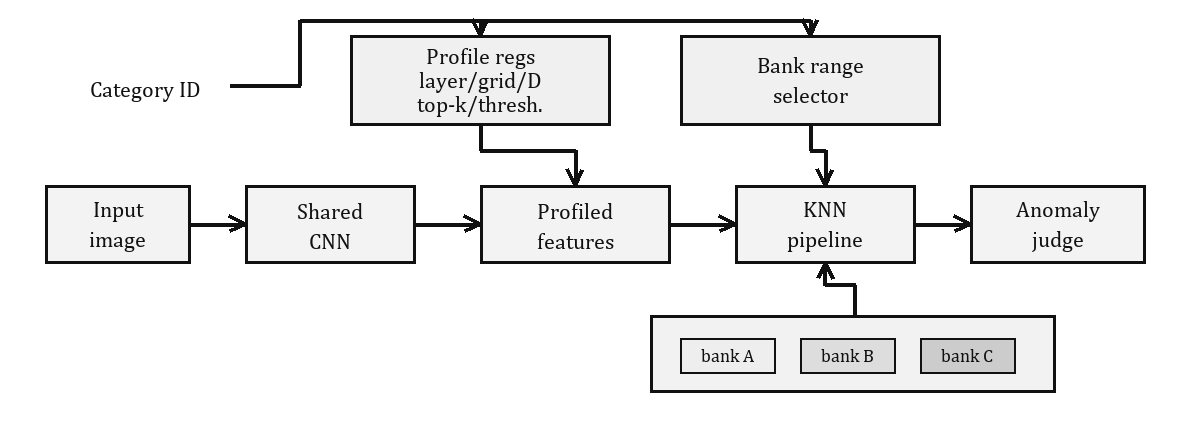
\includegraphics[width=\columnwidth]{figures/system_architecture.png}
\caption{カテゴリ別profile切り替え構成}
\end{figure}
\section*{4. 実験条件}
実験にはMVTec AD[2]の全15カテゴリを用いた。対象カテゴリはbottle，cable，capsule，carpet，grid，hazelnut，leather，metal\_nut，pill，screw，tile，toothbrush，transistor，wood，zipperである。全ての2カテゴリ組み合わせと3カテゴリ組み合わせを評価し，2カテゴリ検品105通り，3カテゴリ検品455通り，合計560通りを対象とした。メモリバンクの構築には正常な学習画像のみを用い，評価には正常画像と欠陥画像の両方を用いた。特徴抽出器にはWideResNet50-2を用いるPatchCore系の実装を用いた。主比較では，全ての比較構成でk-center coreset[1][3]を用い，bank/category=3000にそろえた。

評価指標は，欠陥誤通過率を3\%以下に制約したときの良品通過率である。欠陥誤通過率は欠陥品を正常として通してしまう割合，良品通過率は正常品を正常として通せる割合を意味する。異常判定しきい値は，各構成が欠陥誤通過率3\%以下を満たす範囲で設定した。

比較構成は，(1) デフォルトprofile+共通bank，(2) デフォルトprofile+カテゴリ別bank切り替え，(3) 一つのカテゴリ専用profileを全カテゴリに固定して使う構成+カテゴリ別bank切り替え，(4) カテゴリ別profile+カテゴリ別bank切り替えである。(3)では，各組み合わせで平均良品通過率が最大となる固定profileを採用し，強い単一profile基準として用いた。デフォルトprofileはlayer2+3，grid 14，D=768，top-k 0.010とした。カテゴリ専用profileは，組み合わせ実験の前に単一カテゴリ評価で決定した。bank=12000でprofile候補を探索し，欠陥誤通過率3\%以下の条件で，デフォルトprofileからの良品通過率低下が2ポイント以内の候補を残した。その中でpatch\_count x Dが最小のprofileを各カテゴリの専用profileとして選択した。選択したprofileを表1に示す。

\begin{table}[h]\centering\small
\caption{単一カテゴリ探索で選択したカテゴリ専用profile}
\begin{tabular}{lcccl}\toprule 層 & grid & D & top-k & カテゴリ\\\midrule
layer3 & 14 & 512 & 0.005 & bottle, carpet, hazelnut, leather\\
layer3 & 14 & 512 & 0.005 & metal\_nut, tile, zipper\\
layer3 & 14 & 512 & 0.010 & screw, transistor\\
layer3 & 14 & 512 & 0.020 & capsule\\
layer3 & 14 & 512 & 0.050 & cable\\
layer2+3 & 14 & 768 & 0.005 & grid\\
layer2+3 & 14 & 768 & 0.010 & pill, wood\\
layer2+3 & 14 & 768 & 0.050 & toothbrush\\
\bottomrule\end{tabular}\end{table}
\section*{5. 実験結果}
表2，表3に2カテゴリ検品と3カテゴリ検品の結果を示す。2カテゴリ検品105通りでは，提案するprofile+bank切り替えの平均良品通過率は85.53\%，相対KNN探索量は0.378倍であった。3カテゴリ検品455通りでは，平均良品通過率85.53\%，相対KNN探索量0.252倍であった。提案構成は，良品通過性能を維持しながら，複数カテゴリを一つの検査システムで扱う際の探索活動量を削減した。

共通profileが各カテゴリに十分適合しない組み合わせでは，より大きな改善が得られた。2カテゴリのcable+carpetでは，平均良品通過率が52.59\%から79.99\%へ向上し，KNN探索量は0.333倍となった。3カテゴリのcable+carpet+screwでは，平均良品通過率が37.99\%から66.33\%へ向上し，KNN探索量は0.222倍となった。

\begin{table}[h]\centering\small
\caption{欠陥誤通過率3\%以下での2カテゴリ検品105通りの統計}
\begin{tabular}{lccc}\toprule 構成 & 平均良品 & 最低良品 & NN探索量\\\midrule
共通profile + 共通bank & 80.27\% & 69.30\% & 1.000x\\
カテゴリ別bank切替 & 81.95\% & 71.73\% & 0.500x\\
単一固定profile(best) & 85.01\% & 75.83\% & 0.400x\\
提案: profile+bank切替 & 85.53\% & 76.48\% & 0.378x\\
\bottomrule\end{tabular}\end{table}
\begin{table}[h]\centering\small
\caption{欠陥誤通過率3\%以下での3カテゴリ検品455通りの統計}
\begin{tabular}{lccc}\toprule 構成 & 平均良品 & 最低良品 & NN探索量\\\midrule
共通profile + 共通bank & 79.27\% & 60.43\% & 1.000x\\
カテゴリ別bank切替 & 81.95\% & 65.44\% & 0.333x\\
単一固定profile(best) & 84.49\% & 68.77\% & 0.271x\\
提案: profile+bank切替 & 85.53\% & 70.43\% & 0.252x\\
\bottomrule\end{tabular}\end{table}
\section*{6. 考察}
実験結果から，提案手法ではメモリバンク参照範囲の削減に加えて，profile選択による効果が得られた。カテゴリ別bank切り替えでは探索範囲を減らせるが，提案手法ではさらに，カテゴリごとに特徴層，grid，特徴次元，top-kを選ぶことで平均良品通過率と最低良品通過率が向上した。これは，有効な特徴の取り方がカテゴリに依存することを示している。例えばcableでは大きいtop-kが選択されており，細長い構造や空間的に広がる欠陥を持つカテゴリでは，より多くの高スコアパッチを集約する方が有効である可能性がある。

単一固定profileとの比較は，profile切り替えの必要性を示す。単一固定profileは，各組み合わせに対して最も良い一つのprofileを選ぶ強い基準である。それでも，あるカテゴリ用のprofileを別カテゴリにも強制するため，組み合わせによって性能が不安定になる。提案手法は，カテゴリごとにprofileを割り当てることで，このprofile不一致を避けられる。

近傍探索側の計算量は式(1)で表せる。主比較では各カテゴリのbank数をそろえているため，追加の削減効果はパッチ数や特徴次元などのprofile差から生じる。2カテゴリより3カテゴリで相対KNN探索量が小さくなったことから，対象カテゴリ数が増えるほどカテゴリ別切り替えの効果が表れやすいと考えられる。

\begin{equation}
C_m(S)=\sum_{c\in S}p_c P_{m,c}B_{m,c}D_{m,c},\quad R_m=\frac{C_m(S)}{C_{\rm common}(S)}
\end{equation}
\noindent $P$はパッチ数，$B$は探索bank数，$D$は特徴次元を表す。
\section*{7. FPGA実装に向けた見積もり}
FPGA上では，提案手法の削減をbank開始アドレス，探索長，有効特徴次元，profileレジスタの制御に対応させられる。カテゴリごとに別々のPatchCore回路を用意するのではなく，共通のCNNとKNNデータパスを再利用し，メモリアクセス範囲とループ回数を切り替える構成になる。

FPGA向け見積もりを表4に示す。期待できる効果は，共通CNN前段よりも，KNN探索とメモリアクセスに強く現れる。8bit特徴量を用い，距離計算器が1サイクルに64次元分を処理すると仮定すると，KNNサイクル数とbank読み出し回数は相対KNN探索量に比例する。この見積もりでは，3カテゴリ検品におけるKNN側の活動量は，共通profile構成の約4分の1になる。

今後はprofile制御付きKNNパイプラインを実装し，レイテンシ，メモリ帯域，論理資源，オンチップメモリ，消費電力について，理論見積もりと実測値の差を評価する。KNN演算器の規模は主に距離計算レーン数とメモリポート数に依存し，提案手法で追加されるのはprofileレジスタ，bankアドレスオフセット，小規模な選択回路である。特に，この制御コストがKNNループ数とメモリアクセス削減による利益に対して十分小さいかを確認する。

\begin{table}[h]\centering\small
\caption{bank/category=3000，8bit特徴量，64並列距離計算レーンでのFPGA向け見積もり}
\begin{tabular}{lcccc}\toprule 構成 & cycles/枚 & 比 & 容量 & BRAM\\\midrule
共通profile+bank & 17.88M & 1.000x & 5.57MiB & 1267\\
bank切替 & 7.06M & 0.395x & 5.57MiB & 1267\\
固定profile+bank & 5.52M & 0.309x & 4.34MiB & 988\\
提案切替 & 5.23M & 0.293x & 4.11MiB & 936\\
\bottomrule\end{tabular}\end{table}
\section*{8. まとめ}
本稿では，PatchCore-lite異常検知をFPGAへ実装するためのカテゴリ別profile切り替え構成を検討した。提案の中心は，bank削減そのものではなく，カテゴリごとに有効なprofileを事前に求め，検査時に軽量に切り替える実行方式である。予備実験では，共通profileの基準構成より高い良品通過率と小さい相対KNN探索量を確認した。今後は，FPGA上でモード切り替え型KNNパイプラインを実装し，理論見積もりと実測の差を評価する。

\section*{参考文献}
\noindent [1] K. Rothほか, "Towards Total Recall in Industrial Anomaly Detection," CVPR, 2022.\\
\noindent [2] P. Bergmannほか, "MVTec AD--A Comprehensive Real-World Dataset for Unsupervised Anomaly Detection," CVPR, 2019.\\
\noindent [3] OpenVINO Anomalib Contributors, "PatchCore model documentation," 2026.\\
\end{document}